% ============================================================================
% Networks Decide for Us — Sunbelt 2026
% Session: "Contagion and Diffusion processes through Social Networks"
% Classic-SNA framing: LEAD with the imputation pipeline + structural premium;
% physics demoted to a single teaser slide. ~15 min talk + 5 min Q&A.
% Style replicates the CPIN / "JORNADA REDES" deck.
% Compile: pdflatex presentation-sunbelt26.tex  (run twice)
% ============================================================================
\documentclass[aspectratio=169,11pt]{beamer}

\usepackage[utf8]{inputenc}
\usepackage[T1]{fontenc}
\usepackage{amsmath, amssymb}
\usepackage{graphicx}
\usepackage{booktabs}
\usepackage{array}
\usepackage{xcolor}
\usepackage{colortbl}   % \rowcolor in tables
\usepackage{tikz}
\usepackage{qrcode}
\usetikzlibrary{arrows.meta, positioning, calc, decorations.pathreplacing}

% ---------- Fonts: clean humanist sans, professional math ----------
\usefonttheme{professionalfonts}
\usepackage{helvet}
\renewcommand{\familydefault}{\sfdefault}

% ---------- Colors (matched to the JORNADA deck) ----------
\definecolor{ndred}{RGB}{222,32,38}       % bright red rule
\definecolor{ndreddark}{RGB}{176,22,28}   % darker brick red (subtitles)
\definecolor{ndgreen}{RGB}{0,118,54}      % green reference markers (darker)
\definecolor{ndblue}{RGB}{30,90,200}      % accent blue
\definecolor{ndgray}{RGB}{90,90,90}

% ---------- Strip all Beamer chrome ----------
\setbeamertemplate{navigation symbols}{}
\setbeamercolor{normal text}{fg=black,bg=white}
\setbeamercolor{structure}{fg=ndreddark}
\setbeamertemplate{itemize item}{\color{ndreddark}\textbullet}
\setbeamertemplate{itemize subitem}{\color{ndgray}\textendash}

% ---------- Frame title: centered black title + full-width red rule ----------
\setbeamercolor{frametitle}{fg=black,bg=white}
\setbeamerfont{frametitle}{size=\Large, series=\mdseries}
\setbeamertemplate{frametitle}{%
  \vspace{0.35cm}%
  \begin{center}\insertframetitle\end{center}%
  \vspace{-0.18cm}%
  {\color{ndred}\hrule height 1.1pt}%
}

% ---------- Minimal footline: page number only ----------
\setbeamertemplate{footline}{%
  \hfill{\color{ndgray}\scriptsize\insertframenumber}\hspace{0.5cm}\vspace{0.2cm}}

% ---------- Helper macros ----------
\newcommand{\refn}[1]{{\color{ndgreen}[#1]}}
\newcommand{\emphr}[1]{{\color{ndreddark}\textbf{#1}}}

% Section-divider slide
\newcommand{\sectionslide}[1]{%
  \begin{frame}[plain]
    \vfill
    \begin{center}
      {\Large #1}\\[2pt]
      {\color{ndred}\rule{0.30\textwidth}{1.1pt}}
    \end{center}
    \vfill
  \end{frame}}

% ============================================================================
\title{Networks Decide for Us}
\subtitle{Imputed homophilic networks and the structural premium of diffusion}
\author{Aníbal Olivera M.}
\date{}

\begin{document}

% ---------------------------------------------------------------- 1. TITLE
\begin{frame}[plain]
  \vspace{0.5cm}
  \begin{center}
    
\includegraphics[height=1.0cm]{UDD.png}\hspace{1.2cm}\raisebox{0.25cm}{
\includegraphics[height=0.5cm]{poliCICS.pdf}}
  \end{center}
  \vspace{0.9cm}
  \begin{center}
    {\LARGE \textbf{Networks Decide for Us}}\\[0.5cm]
    {\large \color{ndreddark} Imputed homophilic networks and the structural premium of diffusion}
  \end{center}
  \vspace{1.2cm}
  \begin{center}
    {\normalsize Aníbal Olivera M.}\\[2pt]
    {\footnotesize PhD(c) in Social Complexity Sciences, (CICS)}\\[2pt]
    {\footnotesize with Jorge Fábrega (CICS)}
  \end{center}
  \vfill
  \begin{center}
    {\scriptsize\color{ndgray} Sunbelt 2026 — \emph{Contagion and Diffusion processes through Social Networks}}
  \end{center}
\end{frame}

% ---------------------------------------------------------------- 2. MOTIVATION
% ---------------------------------------------------------------- OVERVIEW
\begin{frame}{The question}
\begin{itemize}
  \item Collective behaviors (innovations, mobilizations) spread as \emphr{adoption cascades} on social networks.
  \vspace{0.2cm}
  \item Most models use \emph{synthetic} topologies and treat agents as simple relays \refn{1}.
  \vspace{0.2cm}
  \item We cluster with people like us. Real networks are shaped by \emphr{multidimensional homophily} \refn{2}.
  \vspace{0.2cm}
  \item Individual \emph{preferences} to adopting behaviors \emphr{can be measured} in surveys.
  \vspace{0.2cm}
  \item Studies often uses peer influence as the only mechanism for adoption.
\end{itemize}
\end{frame}

% ---------------------------------------------------------------- 3b. WHERE WE GO
\begin{frame}{Where we go}
\textbf{Two moves}
\begin{itemize}
  \item \emphr{Impute} plausible whole-networks onto real survey respondents from
        empirical homophily.
  \vspace{0.3cm}
  \item \emphr{Measure} the causal premium of that structure on diffusion.
\end{itemize}
\vspace{0.5cm}
\begin{center}
\fcolorbox{ndred}{white}{\parbox{0.92\textwidth}{\centering
Conditional on \emph{fixed individual characteristics}, does collective behavior depend on the
network's \emphr{shape}, or on \emphr{who sits next to whom}?}}
\end{center}
\end{frame}

% ================================================================ THE MODEL
\sectionslide{The model}

% ---- 4. Rational choice
\begin{frame}{Adoption, part 1 — Rational Choice}
\begin{itemize}
  \item A behavior has an \emph{Intrinsic Utility Level} \emphr{IUL}, $\Gamma\in[0,1]$.
  \item Each person has a \emph{Minimum Utility Requirement} \emphr{MUR}, $q_i\in[0,1]$,
        representing their aversion to adopting the behavior.
\end{itemize}
\vspace{0.1cm}
\begin{center}
An agent adopts on its own iff\quad
\fcolorbox{ndred}{white}{$\;q_i \le \Gamma \;\implies\; a_i = 1\;$}
\end{center}
\vspace{0.15cm}
\begin{center}
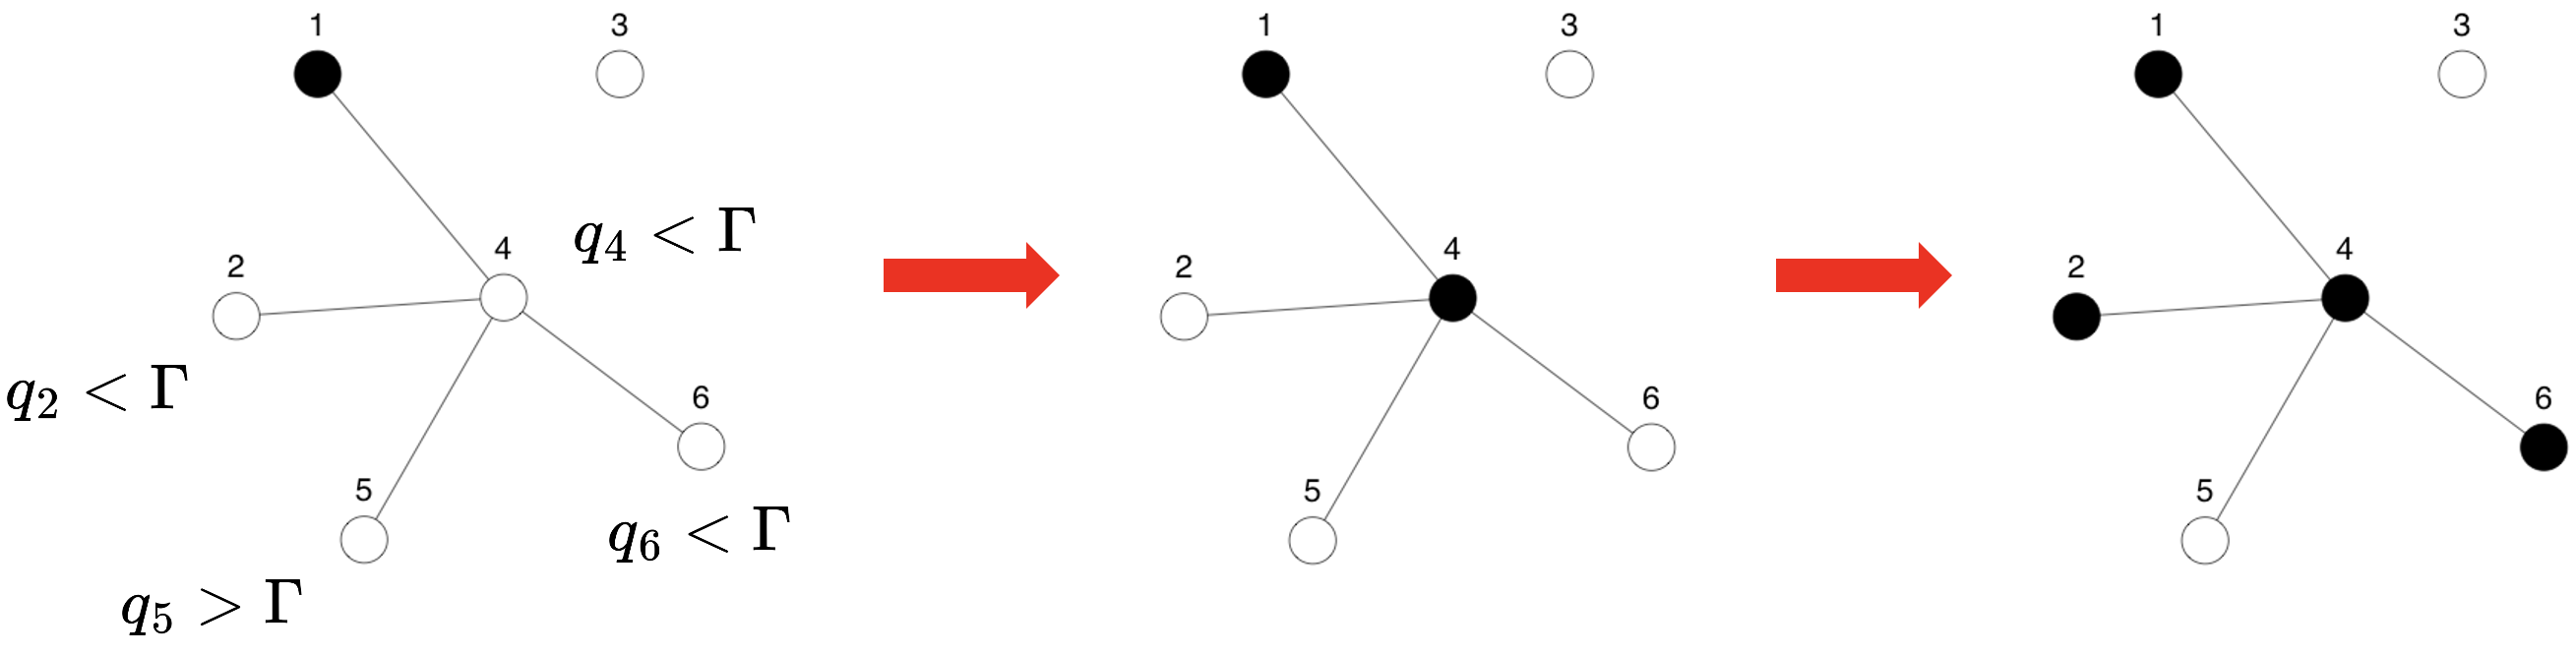
\includegraphics[width=0.95\textwidth]{graph-rational-choice.png}
\end{center}
\end{frame}

% ---- 4. Selective social influence
\begin{frame}{Adoption, part 2 — Selective Social Influence}
Adopt by peer contagion if $\tau_i \le \tilde{E}_i$ \refn{5,6} 
— but only those socially \emph{close} count:
\vspace{0.05cm}
\begin{equation*}
  \tilde{E}_i \equiv \frac{\sum_{j\neq i}\mathbf{X}_{ij}\,\tilde{a}_j}{\sum_{j\neq i}\mathbf{X}_{ij}},
  \qquad
  \tilde{a}_j = 1 \iff a_j = 1 \;\wedge\; U_{ij} \le \sigma\!\left(MSP - d_{ij}\right)
\end{equation*}
\begin{itemize}
  \item There is a Maximum Social Proximity \emphr{MSP} where the limit of influence sits \refn{7}. 
\end{itemize}
\vspace{0.05cm}
\begin{center}
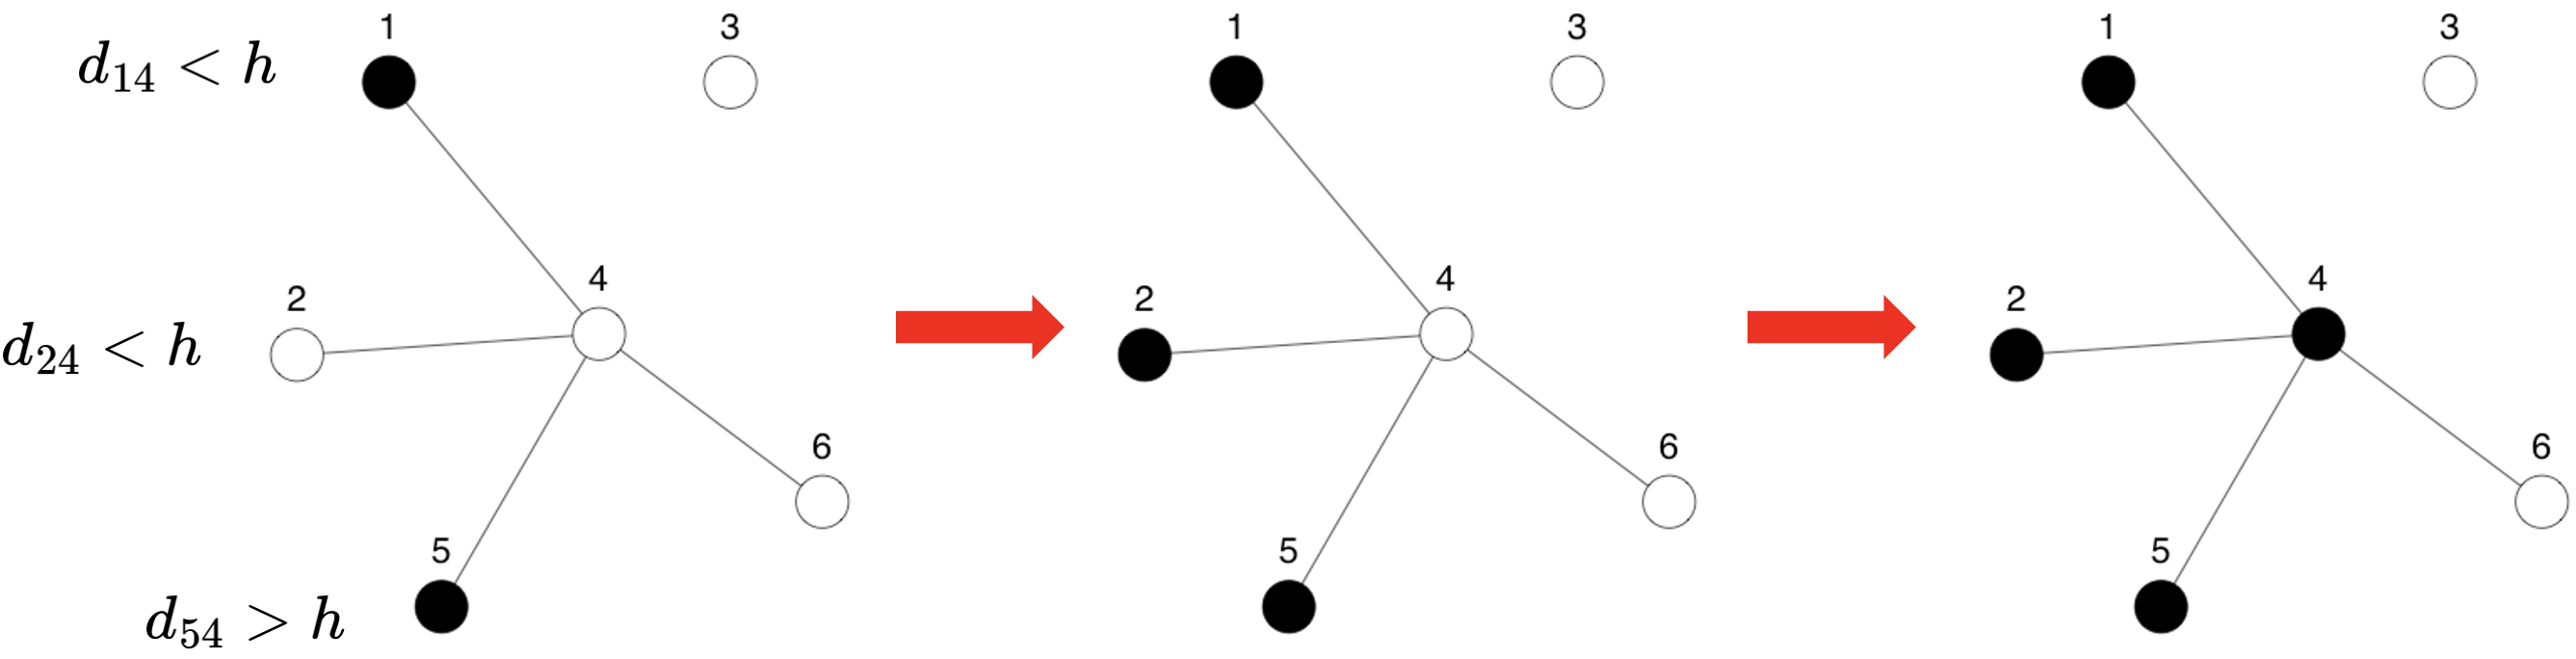
\includegraphics[width=0.9\textwidth]{graph-social-influence.png}
\end{center}
\end{frame}

% ================================================================ PIPELINE
\sectionslide{Imputing structure \& running the model}

% ---- 5. THE PIPELINE (copied from CPIN deck) ----
\begin{frame}{Imputing a network onto a survey}
\begin{center}
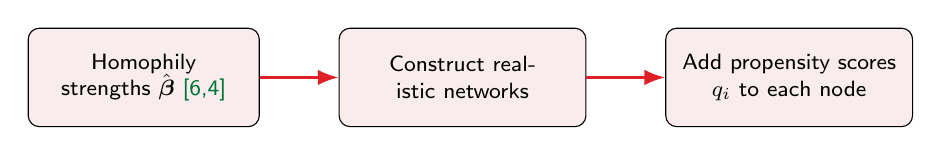
\begin{tikzpicture}[every node/.style={font=\footnotesize}]
  \node[draw,rounded corners,fill=ndreddark!8,text width=2.7cm,align=center,
        minimum height=1.25cm] (a) {Homophily strengths $\hat{\boldsymbol{\beta}}$ \refn{6,4}};
  \node[draw,rounded corners,fill=ndreddark!8,text width=2.9cm,align=center,
        minimum height=1.25cm,right=1.0cm of a] (b) {Construct realistic networks};
  \node[draw,rounded corners,fill=ndreddark!8,text width=2.9cm,align=center,
        minimum height=1.25cm,right=1.0cm of b] (c) {Add propensity scores $q_i$ to each node};
  \draw[-{Latex},ndred,line width=1pt] (a)--(b);
  \draw[-{Latex},ndred,line width=1pt] (b)--(c);
\end{tikzpicture}
\end{center}
\vspace{0.2cm}
\begin{columns}[c]
\column{0.52\textwidth}
\footnotesize
Tie probability is a function of social distance (age, sex, education, race, religion):
\vspace{0.2cm}
\begin{equation*}
  \mathrm{logit}\,\Pr(Y_{ij}=1)=\alpha+\boldsymbol\beta^\top \mathbf{d}_{ij}
\end{equation*}

$\hat{\boldsymbol\beta}$ comes from GSS confidant data \refn{6}; propensities $q_i$ come from
real survey answers (innovation, collective action).
\column{0.48\textwidth}
\centering
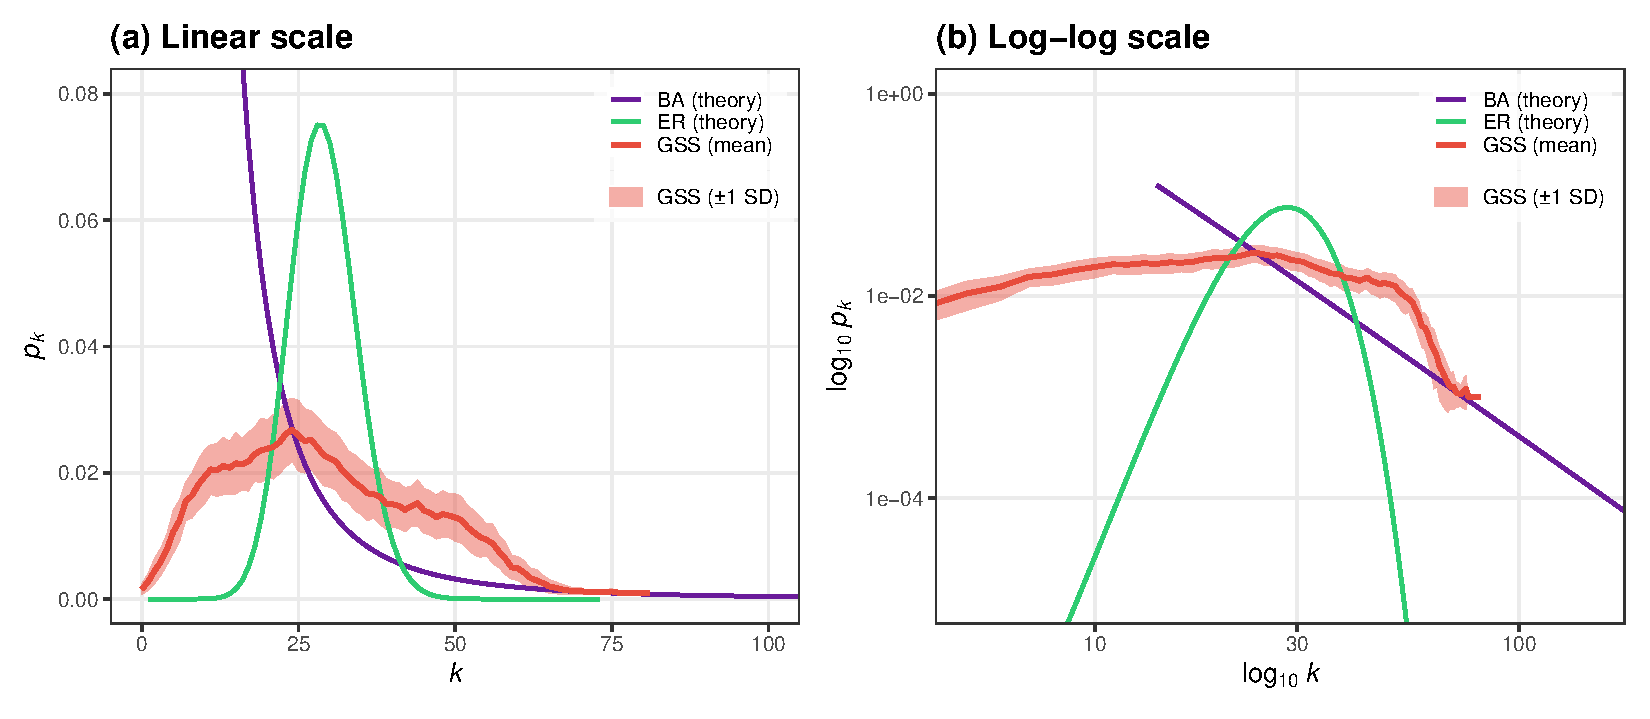
\includegraphics[width=0.92\linewidth]{../../plots/02_GSS_network_ergm_tests/GSS_degree_dist.pdf}\\
{\scriptsize Right-skewed degree structure that Erdös-Rényi / Barabási-Albert models fail to match jointly.}
\end{columns}
\end{frame}

% ---- NEW (pt 2.1): the two counterfactual baselines ----
\begin{frame}{Two ways to ``break'' the network}
\begin{center}
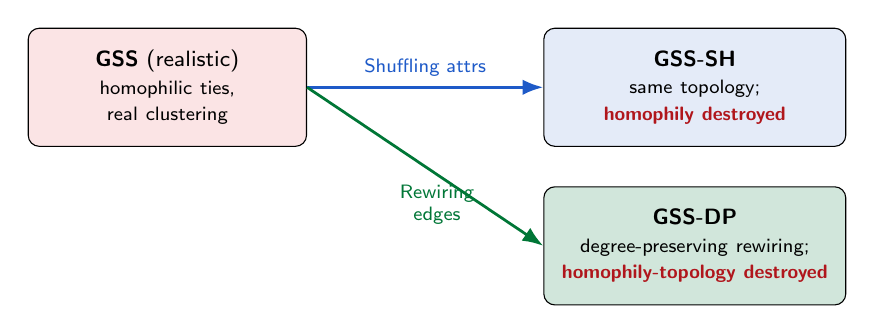
\begin{tikzpicture}[every node/.style={font=\footnotesize,align=center}, node distance=0.7cm]
  \node[draw,rounded corners,fill=ndred!12,text width=3.3cm,minimum height=1.5cm] (gss)
    {\textbf{GSS} (realistic)\\[2pt]\scriptsize homophilic ties,\\ real clustering};
  \node[draw,rounded corners,fill=ndblue!12,text width=3.6cm,minimum height=1.5cm,right=3.0cm of gss] (sh)
    {\textbf{GSS-SH}\\[2pt]\scriptsize same topology;\\ \emphr{homophily destroyed}};
  \node[draw,rounded corners,fill=ndgreen!18,text width=3.6cm,minimum height=1.5cm,below=0.5cm of sh] (dp)
    {\textbf{GSS-DP}\\[2pt]\scriptsize degree-preserving rewiring;\\ \emphr{homophily-topology destroyed}};
  \draw[-{Latex},ndblue,line width=1pt] (gss.east) -- node[above,font=\scriptsize]{Shuffling attrs} (sh.west);
  \draw[-{Latex},ndgreen,line width=1pt] (gss.east) -- node[below,font=\scriptsize,pos=0.55]{Rewiring\\ edges} (dp.west);
\end{tikzpicture}
\end{center}
\vspace{0.1cm}
\begin{center}\small
\emph{GSS} vs \emph{GSS-SH} isolates \emphr{homophily}; \emph{GSS-SH} vs \emph{GSS-DP}
 how much \emphr{topology} adds.
\end{center}
\end{frame}

% ---- 6a. RESULT 2 moved up: higher-order topology (family B) ----
\begin{frame}{What is destroyed? — topology}
\centering
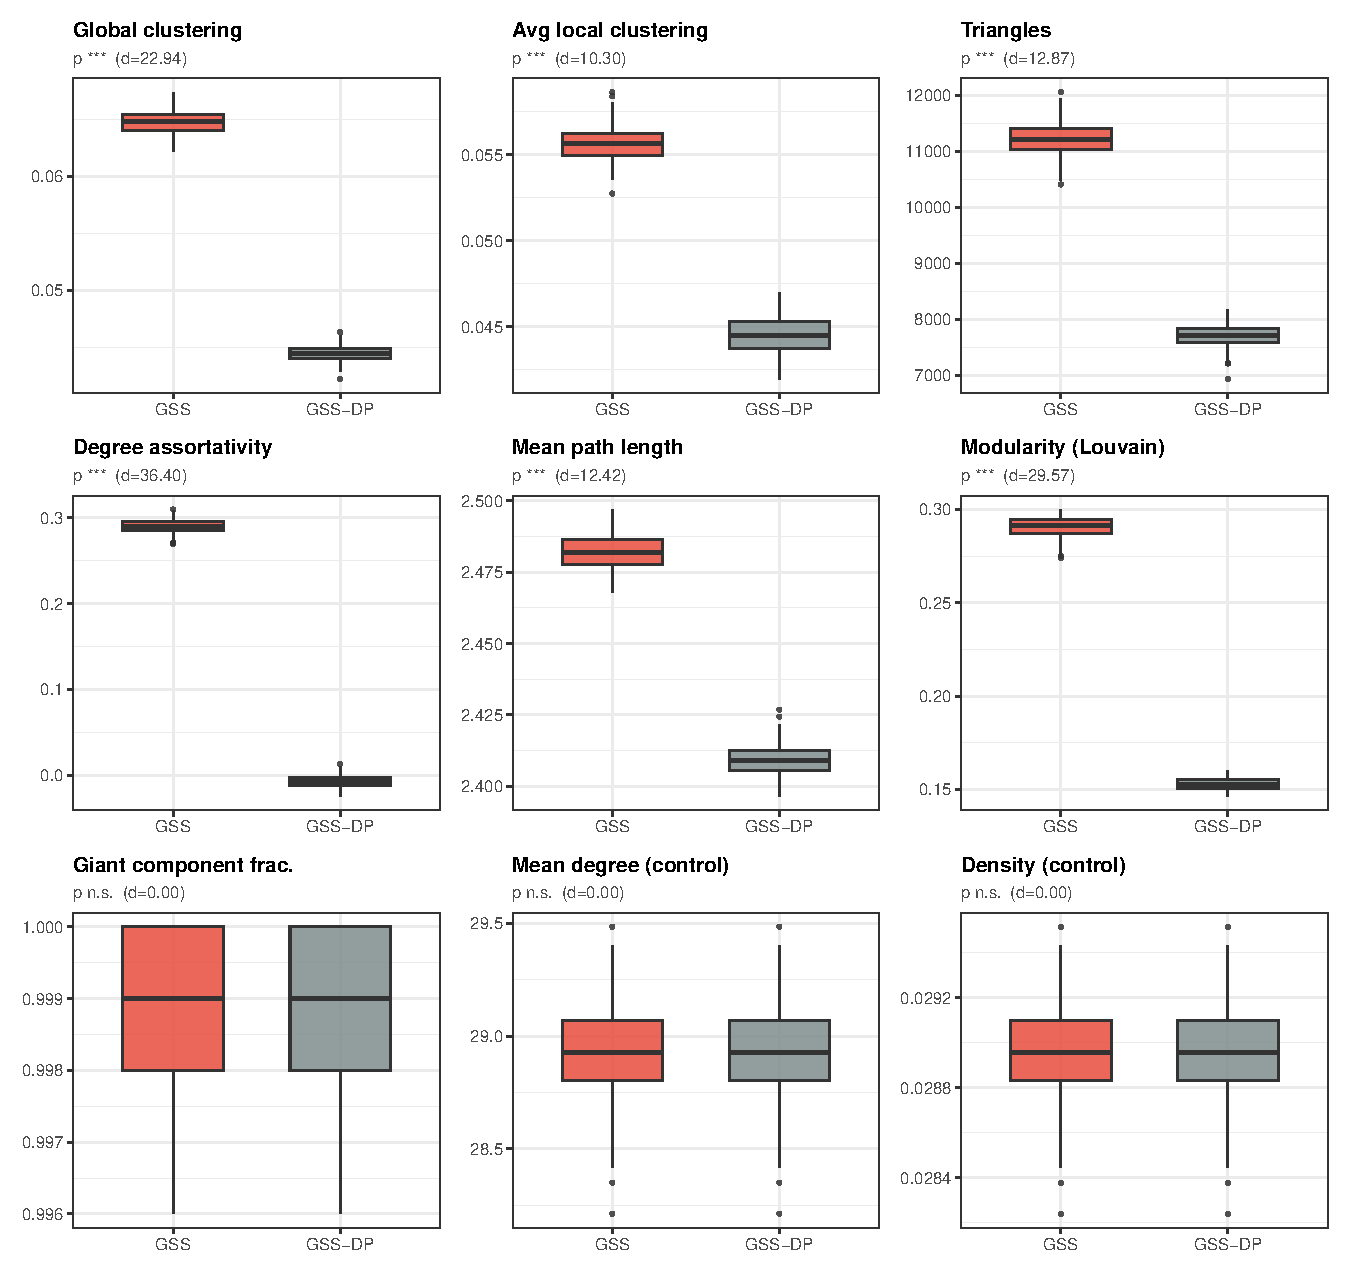
\includegraphics[height=0.745\textheight]{../../playground/checks-claude/plots/structural_diagnosis_B.pdf}\\[2pt]
{\footnotesize Topology statistics across 100 networks each. \emphr{GSS and GSS-SH} are
identical; only \emphr{GSS-DP}
degrades them: clustering $-31\%$, triangles $-31\%$, modularity $-47\%$.}
\end{frame}

% ---- 6b. RESULT 2: homophily (family C) ----
\begin{frame}{What is destroyed? — homophily}
\centering
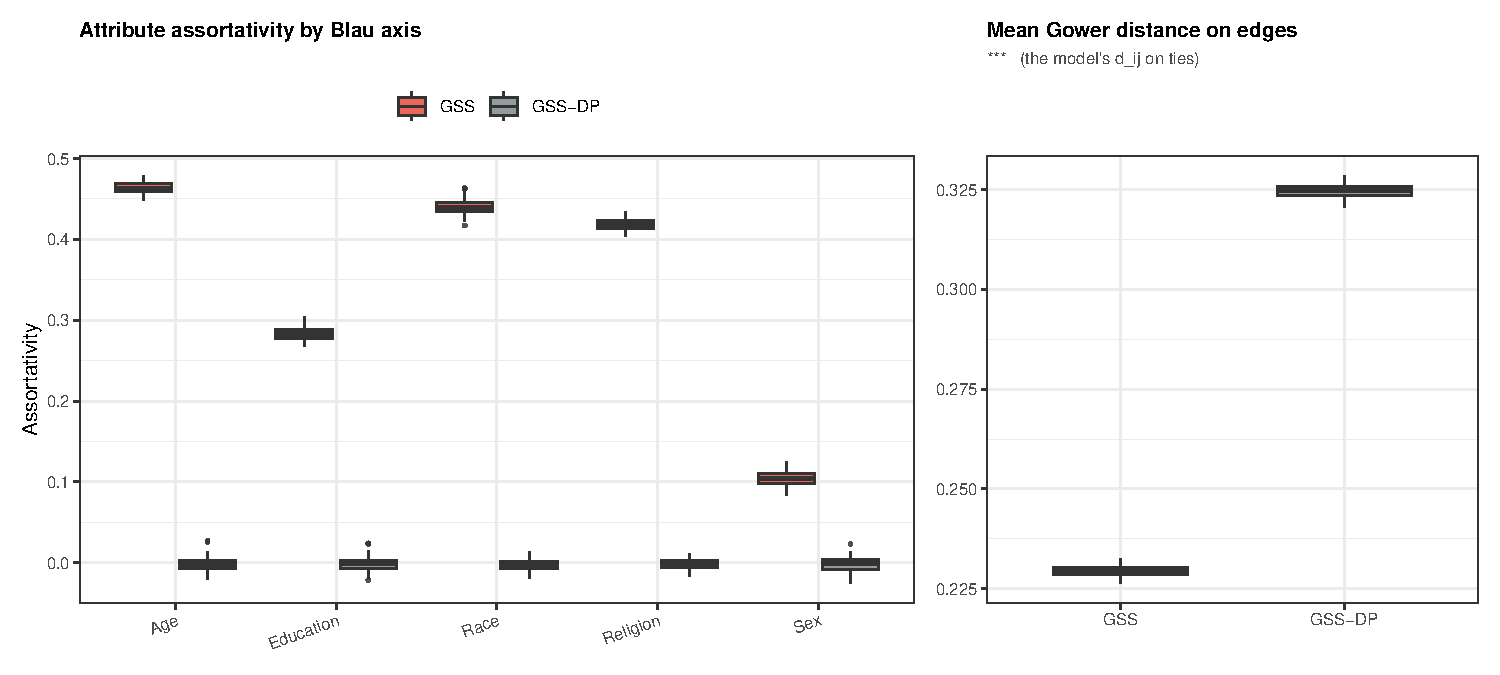
\includegraphics[width=0.99\textwidth]{../../playground/checks-claude/plots/structural_diagnosis_C.pdf}\\[6pt]
{\footnotesize \emphr{both GSS-SH and GSS-DP annihilate homophily.} \\ 
So the shuffle destroys \emph{homophily only}, the rewiring destroys \emph{both}.}
\end{frame}

% ---- 6c. Simulation design ----
\begin{frame}{Comprehensive simulation design}
Hybrid social contagion via \texttt{netdiffuseR} \refn{7}, over plausible \emphr{GSS} vs. \\
\emphr{GSS-DP} (degree-preserving) and \emphr{GSS-SH} (shuffled attributes) networks.
\vspace{0.2cm}
\begin{itemize}
  \item \textbf{IUL} ($\Gamma$): 41 levels $[0,1]$. \quad \textbf{MSP} ($h$): 13 levels $[0,1]$.
  \item \textbf{Thresholds} $\tau_i\sim\mathcal{N}(\mu,\sigma)$: $\mu\in\{.3,.4,.5,.6\}$, $\sigma\in\{.08,.12,.16,.20\}$.
  \item \textbf{Seeding}: random, central, marginal, closeness, eigenvector.
\end{itemize}
\vspace{0.2cm}
\begin{center}
Total: $\;41\times13\times4\times4\times5\times \text{(runs)} \;\approx\; \emphr{$4\times10^{6}$ simulations}$
\end{center}
\vspace{0.2cm}
We then fit \emph{Big Additive Models} (BAM) to isolate the structural effect:
\begin{equation*}
  \mathrm{logit}\big[\mathbb{E}(\Phi)\big]=\beta_0+\mathbf{Z}\boldsymbol\beta
  +\beta_{\text{DP}}\,\mathbb{I}_{\text{DP}}+\beta_{\text{SH}}\,\mathbb{I}_{\text{SH}}+s(\mathrm{IUL},\mathrm{MSP})
\end{equation*}
\end{frame}

% ================================================================ RESULTS
\sectionslide{Results}

% ---- 7a. RESULT 1: adoption dynamics (top row of figure1; crop bottom row) ----
\begin{frame}{Result 1 — How adoption plays out}
\centering
% crop: keep only the TOP row (Total / Rational / Social adoption); drop the bottom row
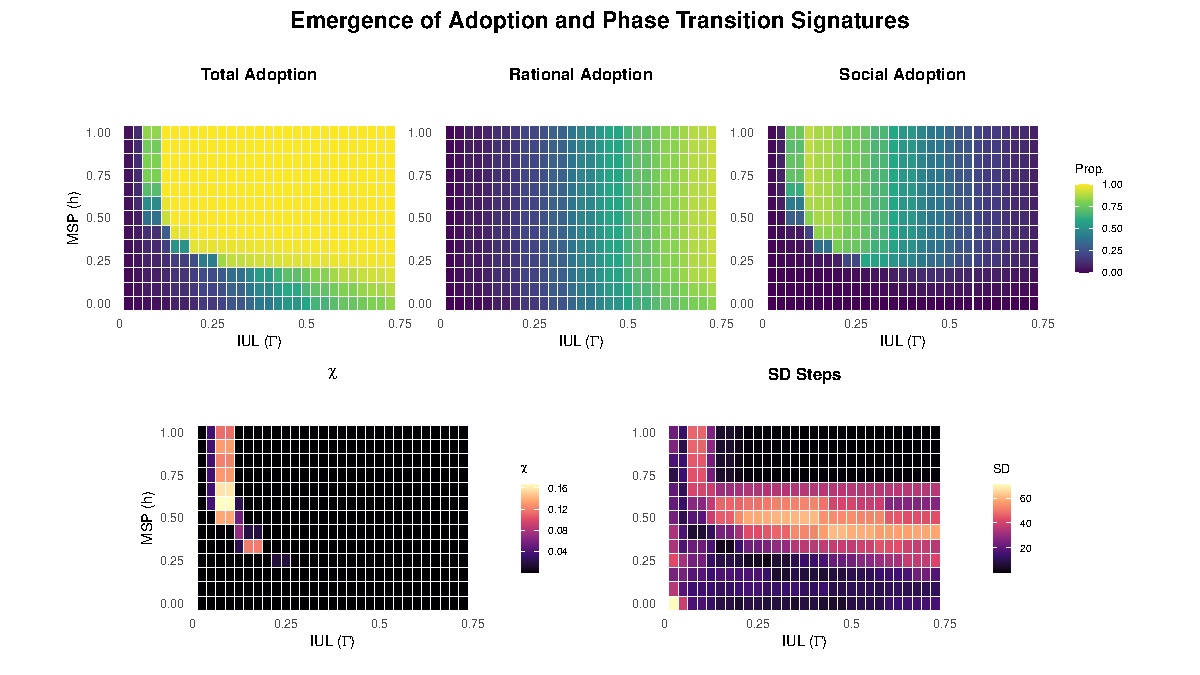
\includegraphics[trim={0 5.25cm 0 1.1cm}, clip, width=0.98\textwidth]{../abstract-sn26/figure1_5panels_GSS.pdf}\\[4pt]
{\footnotesize Mean adoption over the attractiveness (IUL) -- openness (MSP) plane. \\
\emphr{Rational} adoption grows with attractiveness; \emphr{social} adoption is more
complex, so total adoption stays high over a wide region \emph{even when the behavior is
barely attractive}.}
\end{frame}

% ---- 7b. RESULT 2 (pt 3, slide 1): total adoption drops ----
\begin{frame}{Result 2 — Breaking structure cuts adoption}
\begin{columns}[c]
\column{0.5\textwidth}
How are the adoption results when we compare with the broken versions? 
\begin{center}
\renewcommand{\arraystretch}{1.5}
{\small
\begin{tabular}{@{}lcc@{}}
\toprule
\textbf{vs.\ GSS} & OR & odds drop \\
\midrule
\rowcolor{ndblue!12} GSS-SH (shuffle) & 0.465 & \emphr{$-53\%$} \\
\rowcolor{ndgreen!12} GSS-DP (rewire) & 0.432 & \emphr{$-57\%$} \\
\bottomrule
\end{tabular}}
\end{center}
\vspace{0.3cm}
\small Same individuals, same propensities, but adoption
falls by more than half. \\
\vspace{0.2cm} 
In both the \emph{homophily is destroyed} - lack of \emphr{echo chambers}
\column{0.5\textwidth}
\centering
\renewcommand{\arraystretch}{1.1}
{\scriptsize
\begin{tabular}{@{}lcc@{}}
\toprule
\textbf{Total adoption (GSS)} & Estimate & OR \\
\midrule
(Intercept) & $6.384^{***}$ & --- \\
$\tau_{\text{mean}}$ & $-6.784^{***}$ & --- \\
$\tau_{\text{sd}}$ & $5.820^{***}$ & --- \\
\addlinespace
\multicolumn{3}{@{}l}{\textit{Seeding (ref: Random)}}\\
\quad Central & $0.130^{***}$ & 1.139 \\
\quad Closeness & $0.130^{***}$ & 1.138 \\
\quad Eigenvector & $0.129^{***}$ & 1.138 \\
\quad Marginal & $-0.073^{***}$ & 0.930 \\
\addlinespace
\multicolumn{3}{@{}l}{\textit{Network (ref: GSS)}}\\
\quad GSS-SH & $\mathbf{-0.766}^{***}$ & \textbf{0.465} \\
\quad GSS-DP & $\mathbf{-0.840}^{***}$ & \textbf{0.432} \\
\midrule
\multicolumn{3}{@{}l}{Dev.\ expl.: 82.6\%\quad $N\approx5.1\times10^{6}$}\\
\bottomrule
\end{tabular}}
\\[3pt]{\scriptsize $^{***}p<0.001$. OR $=\exp(\beta)$.}
\end{columns}
\end{frame}

% ---- 7c. RESULT 2 (pt 3, slide 2): homophily alone reproduces most of the drop ----
\begin{frame}{Result 2 — Homophily alone reproduces most of the drop}
\begin{columns}[c]
\column{0.52\textwidth}
The two models compare like this:
\vspace{0.25cm}
\begin{center}
\fcolorbox{ndred}{white}{\parbox{0.96\linewidth}{\centering
\textcolor{ndblue}{GSS-SH \emph{$-53\%$}} \;\; homophily destroyed\\[4pt]
\textcolor{ndgreen}{GSS-DP \emph{$-57\%$}} \; homophily \emph{and} topology}}
\end{center}
\vspace{0.3cm}
Breaking \emph{only} homophily — keeping the topology — already recovers
\emphr{$\sim$91\%} of the full drop.
\vspace{0.4cm}

$\Rightarrow$ \emphr{homophily is doing most of the work}.
\column{0.45\textwidth}
\centering
% simple decomposition bar: homophily (SH) vs the small topology remainder
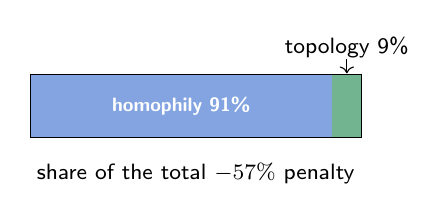
\begin{tikzpicture}[font=\footnotesize]
  \def\W{4.2}
  \fill[ndblue!55] (0,0) rectangle (\W*0.913,0.8);
  \fill[ndgreen!55] (\W*0.913,0) rectangle (\W,0.8);
  \draw (0,0) rectangle (\W,0.8);
  \node[white,font=\scriptsize\bfseries] at (\W*0.913/2,0.4) {homophily 91\%};
  \node[font=\footnotesize] at (\W*0.957,1.15) {topology 9\%};
  \draw[->] (\W*0.957,1.0) -- (\W*0.957,0.82);
  \node[font=\footnotesize] at (\W/2,-0.45) {share of the total $-57\%$ penalty};
\end{tikzpicture}
\end{columns}
\end{frame}

% ================================================================ CLOSE
% ---- conclusions ----
\begin{frame}{Conclusions}
\begin{enumerate}
  \item \textbf{A method:} you can build \emphr{realistic}, simulable whole-networks for survey respondents out of \emphr{empirical homophily}.
  \vspace{0.1cm}
  \item \textbf{Three findings:} \\
  \hspace{0.5cm} 1. Social influence explains adoption even for non-attractive behaviors*. \\
  \hspace{0.5cm} 2. Empirical structure yields a
        \emphr{$+57\%$ adoption premium}. \\
  \hspace{0.5cm} 3. In realistic social networks, topology it not all: \emphr{who sits next to whom} is critical.
  \vspace{0.1cm}
  \item \textbf{A mechanism:} what's doing the work is \emphr{homophily}, not the abstract topology.
\end{enumerate}
\vspace{0.2cm}
\begin{center}\small
\emph{Where a behavior ends up is not the sum of individual preferences}, \\
but it's \emphr{governed by the structure of our real ties.}
\end{center}
\end{frame}

% ---- references ----
\begin{frame}{References}
\footnotesize
\begin{enumerate}\itemsep1.2pt
  \item McPherson, Smith-Lovin \& Cook (2001). Birds of a Feather. \emph{Annu. Rev. Sociol.} 27.
  \item Goldberg (2021). Associative Diffusion \& the Pitfalls of Structural Reductionism. \emph{ASR} 86(6).
  \item Granovetter (1978). Threshold Models of Collective Behavior. \emph{AJS} 83(6). / Valente (1996). \emph{Soc. Networks} 18(1).
  \item McPherson \& Smith (2019). Network Effects in Blau Space. \emph{Socius} 5.
  \item Bradley \& Terry (1952). Rank Analysis of Incomplete Block Designs. \emph{Biometrika} 39.
  \item Smith, McPherson \& Smith-Lovin (2014). Social Distance in the U.S. \emph{ASR} 79(3).
  \item Vega Yon, Olivera M.\ \& Valente (2025). \texttt{netdiffuseR}. \emph{Zenodo}.
  \item Macy \& Evtushenko (2020). Threshold Models of Collective Behavior II. \emph{Sociological Science} 7.
  \item Sethna (2021). \emph{Statistical Mechanics: Entropy, Order Parameters, and Complexity}. Oxford UP.
\end{enumerate}
\end{frame}

% ---- 14. thanks + QR ----
\begin{frame}[plain]
  \vfill
  \begin{center}
    {\Large Thanks!}\\[2pt]
    {\color{ndred}\rule{0.30\textwidth}{1.1pt}}\\[0.6cm]
    \qrcode[height=2.2cm]{https://doi.org/10.5281/zenodo.19360209}\\[0.3cm]
    {\footnotesize Scan: preprint draft (Zenodo)}\\[5pt]
    {\footnotesize \texttt{an.oliveram@udd.cl} $\;\cdot\;$ \texttt{aoliveram.cl}}\\[6pt]
    \parbox{0.82\textwidth}{\centering\scriptsize\color{ndgray}
      Olivera Morales, A., Fábrega, J., \& Valente, T. (2026). \emph{Networks Decide for Us:
      Emergence of Adoption in Homophily-Imputed Social Topologies}. Zenodo.
      \texttt{https://doi.org/10.5281/zenodo.19360209}}
  \end{center}
  \vfill
\end{frame}

% ---- BACKUP / only if time remains: the SHAPE of change + universality ----
\begin{frame}{Backup — the \emph{shape} of change also differs}
\begin{columns}[c]
\column{0.5\textwidth}
\small
Beyond \emph{how much}, structure governs \emph{how} adoption tips.
\begin{equation*}
  \chi\sim|MSP-MSP_c|^{-\gamma}
\end{equation*}
\begin{equation*}
  \Phi\sim|IUL-IUL_c|^{-\delta}
\end{equation*}

And here the \emph{other} structural property does the work: \emphr{GSS-SH keeps
universality ($\gamma\!\approx\!1$)} even though it has no homophily — only \emphr{GSS-DP},
which destroys the \emph{topology}, loses it \refn{9}.
\vspace{0.2cm}

\renewcommand{\arraystretch}{1.15}
{\footnotesize
\begin{tabular}{@{}lccc@{}}
\toprule
Suscept. $\gamma$ & \textbf{GSS} & \textbf{GSS-SH} & \textbf{GSS-DP} \\
\midrule
mean & $\approx 0.91$ & $\approx 1.08$ & $\approx 3.9$ \\
\bottomrule
\end{tabular}}\\[5pt]
{\scriptsize \emphr{Double dissociation:} homophily $\to$ \emph{volume} (Result 2);
topology $\to$ \emph{continuity} (here).}
\column{0.5\textwidth}
\centering
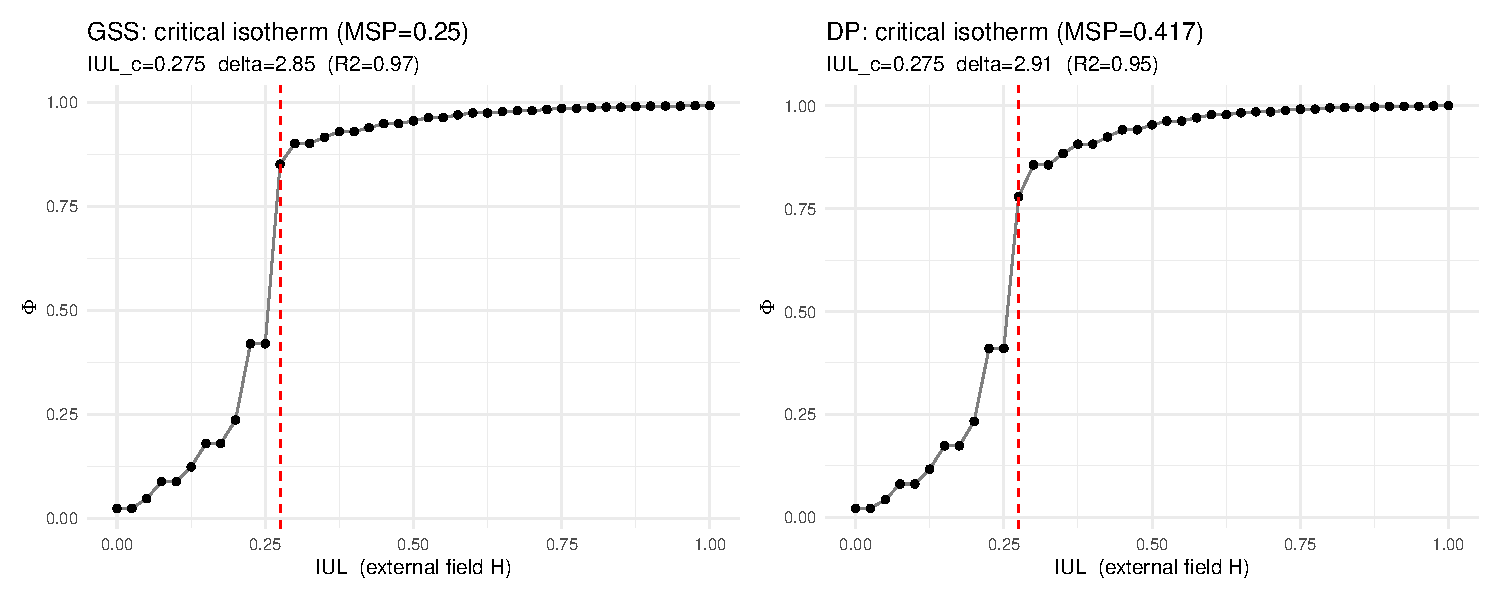
\includegraphics[width=\linewidth]{../../playground/checks-claude/plots/camino_H_critical_isotherm.pdf}\\
{\scriptsize Critical isotherms $\Phi(\mathrm{IUL})$ at $MSP{=}MSP_c$: along the field axis
\emph{both} give $\delta\!\approx\!3$; only $\gamma$ (the openness axis) discriminates.}
\end{columns}
\end{frame}

% ---- TECHNICAL DETAILS (backup) ----
\begin{frame}{Technical details}
\begin{itemize}
  \item \textbf{Social distance} $d_{ij}\in[0,1]$ — Gower distance over the Blau-space
        attributes (race, sex, religion, age, education):
\end{itemize}
\begin{equation*}
  d_{ij} = \frac{1}{p}\sum_{k=1}^{p} \delta_{ij}^{k},
  \qquad
  \delta_{ij}^{k} =
  \begin{cases}
    \mathbb{1}\!\left[x_i^{k}\neq x_j^{k}\right] & \text{categorical } (\text{race, sex, religion})\\[4pt]
    \dfrac{\big|x_i^{k}-x_j^{k}\big|}{\max_k - \min_k} & \text{numeric } (\text{age, education})
  \end{cases}
\end{equation*}
\vspace{0.3cm}
\footnotesize
* The idiosyncrasy that drives this is
\emphr{measured preference} and \emphr{realistic structure}, not stochastic noise
(Macy \& Evtushenko \refn{8}).
\end{frame}

\end{document}
